\documentclass[12pt]{article}
\usepackage[a4paper]{geometry}
\usepackage[myheadings]{fullpage}
\usepackage{fancyhdr}
\usepackage{lastpage}
\usepackage{graphicx, wrapfig, subcaption, setspace, booktabs}
\usepackage{amsfonts,dcolumn}
\usepackage[T1]{fontenc}
\usepackage[font=small, labelfont=bf]{caption}
\usepackage{fourier}
\usepackage[protrusion=true, expansion=true]{microtype}
\usepackage[english]{babel}
\usepackage{sectsty}
\usepackage{url, lipsum}
\usepackage{listings}
\usepackage{float}

\lstdefinestyle{customc}{
  belowcaptionskip=1\baselineskip,
  breaklines=true,
  frame=L,
  xleftmargin=\parindent,
  language=Python,
  showstringspaces=false,
  basicstyle=\footnotesize\ttfamily,
  keywordstyle=\bfseries\color{green!40!black},
  commentstyle=\itshape\color{purple!40!black},
  identifierstyle=\color{blue},
  stringstyle=\color{orange},
}


\newcommand{\HRule}[1]{\rule{\linewidth}{#1}}
\onehalfspacing
\setcounter{tocdepth}{5}
\setcounter{secnumdepth}{5}

%-------------------------------------------------------------------------------
% HEADER & FOOTER
%-------------------------------------------------------------------------------
\pagestyle{fancy}
\fancyhf{}
\setlength\headheight{15pt}
\fancyhead[L]{Intro to Computational and Data Science}
\fancyhead[R]{Stony Brook University}
\fancyfoot[R]{Page \thepage\ of \pageref{LastPage}}
%-------------------------------------------------------------------------------
% TITLE PAGE
%-------------------------------------------------------------------------------

\begin{document}
\begin{sloppypar}
\title{ \LARGE \textsc{AMS561 Final Project}
		\\ [2.0cm]
		\HRule{0.5pt} \\
		\LARGE \textbf{\uppercase{Graduate Admission Analysis}}
		\HRule{2pt} \\ [0.5cm]
		\normalsize \today \vspace*{5\baselineskip}}

\date{}


\author{\begin{tabular}{rl}
  \textbf{Name:} &Yifan Zhai\\
  \textbf{SBID:}  &112360276\\
  \textbf{Department:} & Technolog \& Society\\
  \textbf{Instructor:} & Robert Harrison
\end{tabular}}

\maketitle
\thispagestyle{empty}
\newpage
\setcounter{page}{1}
\tableofcontents
\newpage


\section{Introduction}

\subsection{Data Resource}
This project uses a Graduate Admission [1] dataset which is inspired by the UCLA Graduate Dataset in an Indian perspective. The dataset is public and available on \texttt{kaggle}. 

The dataset has 400 entries and 9 variables with no NULL value. The first variable is the serial number of each student, which is not correlated with the chance of admission and I set it as the index of dataset. Other variables are  considered important during the application for Masters Programs, including : 1. GRE Scores ( out of 340 ) 2. TOEFL Scores ( out of 120 ) 3. University Rating ( out of 5 ) 4. Statement of Purpose (out of 5) 5. Letter of Recommendation Strength ( out of 5 ) 6. Undergraduate GPA ( out of 10 ) 7. Research Experience ( either 0 or 1 ) 8. Chance of Admit ( ranging from 0 to 1). Figure 1 below shows first few rows of the dataset to give you a quick understanding of the dataset.
\begin{figure}[H]
    \centering
    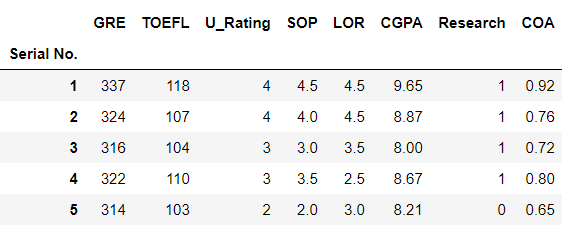
\includegraphics{head.png}
    \caption{First five rows of the dataset}
\end{figure}


\subsection{objective}

To apply for a master's degree is a very expensive and intensive work. There are many motley intermediary agents charges a lot to assist students applying for the graduate school. This project aims to generate a fair and sound analysis report to find the most relevant factors and their relationship with the chance of admission. Besides, students could use my models to test their capacities and choose the most fitting graduate schools.\\
There are three outcomes for this project. Firstly, the distribution of students' test scores and other variables. Secondly, the most influential components. Lastly, the prediction of the probability that a student can be admitted to the college. Other details will be presented in the following sections. 

\section{Methods}

In this section, the techniques and tools used in the project will be covered in detail. 

\subsection{Language \& Environment}

This project is built in Jupyter Notebook in \texttt{Python 3}. Jupyter Notebook is an open-source web application supporting live code and clean text. Python 3 is an object-oriented high-level programming language released in 2008 [2]. I apply data cleaning, transformation, statistical modeling, data visualization and machine learning techniques to the dataset.
\subsection{Packages \& Tools}

Packages imported includes: Numpy, Pandas, Matplot, Seaborn and scikit-learn.

Numpy is a fundamental package for scientific computing, I use its "array" in this project. Pandas, derived from "panel data", is a software library written for the Python programming language for data manipulation and analysis [3]. This project uses pandas to load and manipulate the dataset. Seaborn is a Python data visualization library based on matplotlib [5], it has many strong tools including \texttt{boxplot}, \texttt{heatmap} and \texttt{pairplot}.

Scikit-learn, short for sklearn, is a machine learning package in Python with many efficient tools for data mining. It is built on NumPy, SciPy and matplotlib [4]. The tools used in our project incudes: 
\begin{enumerate}
    \item model\_selection: dividing the dataset into training set and test set.
    \item linear\_model: building linear model and predict on the test dataset.
    \item metrics: building confusion matrix, calculating precision score, recall score, accuracy score and $r^2$ score. 
    \item trees: including decision tree regression model and decision tree classification model
    \item ensemble: including random foreset regression model and random forest classification model
    \item neighbors: building k nearest neighbors model, which is supervised learning
    \item svm: support vector machine is a classification model
\end{enumerate}

\section{Results}

\subsection{Correlation Between Columns}

Firstly, I use the \texttt{heatmap} (Figure 2) to visualize the correlation between every two columns so that we can get a primary cognition of the relationship in the dataset.

\begin{figure}[H]
    \centering
    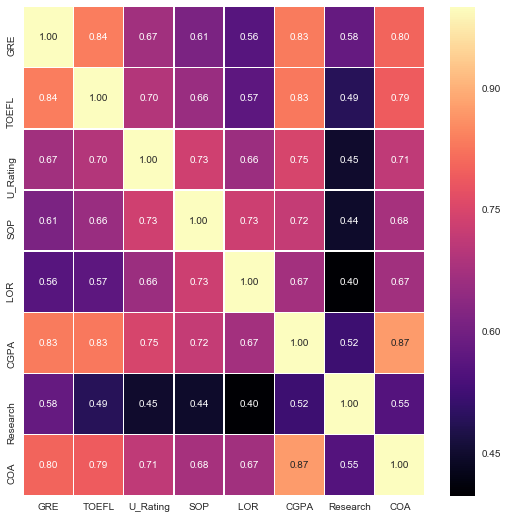
\includegraphics[scale = 0.8]{corr_heatmap.png}
    \caption{Correlation Heatmap }
\end{figure}
In the heatmap, it is obvious that 3 most important features for admission to the Master are CGPA ("College GPA"), GRE SCORE and TOEFL SCORE. Therefore, we want to go for more details about the relationship between these three variables and chance of admission. The pair plot (Figure 3) with the students having research experience or not is presented.

\begin{figure}[H]
    \centering
    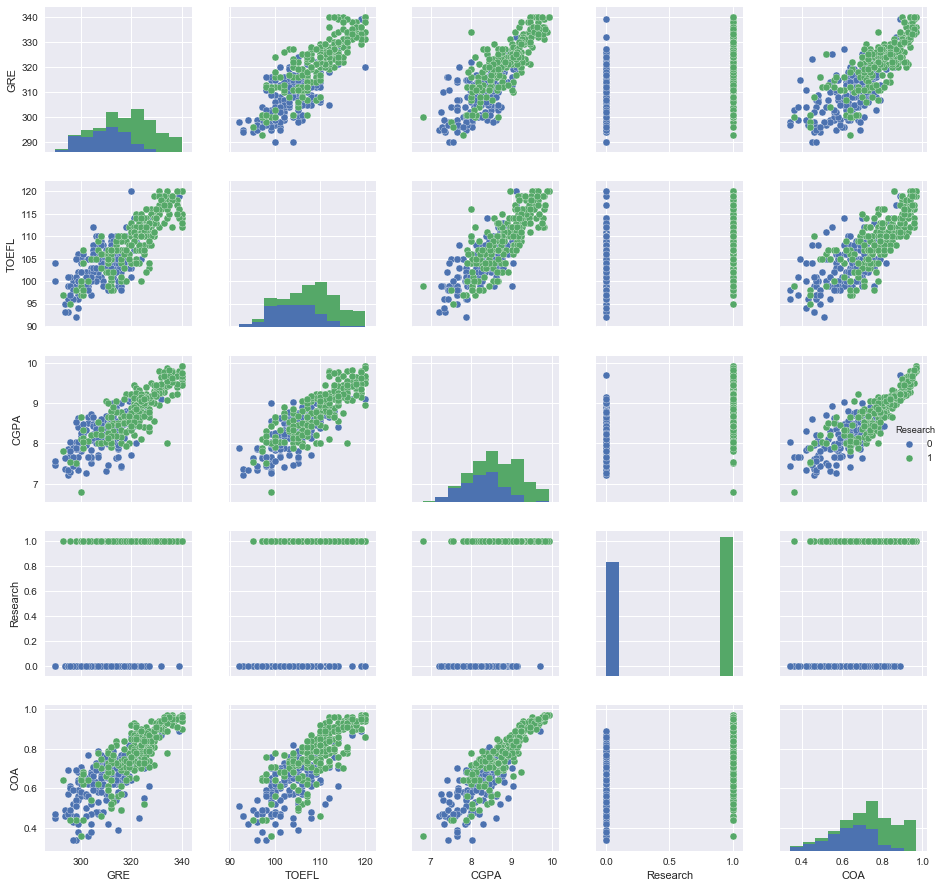
\includegraphics[scale = 0.46]{pair_plot.png}
    \caption{Pair Plot}
\end{figure}

From the pair plot, GRE, TOEFL and CGPA appears to be positive linear related to the Chance of Admission. Therefore, we should consider using linear regression model afterwards. Besides, students with research experience tend to have higher GRE, TOEFL Score, CGPA and higher Chance of Admission eventually. Before building models, let's take a look into the distribution of these three important variables and Chance of Admission.\\
From the plots below, the GRE score is normally distributed and most students have GRE score between 310 and 325. The median TOEFL score is about 106 and college GPA also has a bell-shaped curve. As normal distribution is applied to the attributes of students, the student in the upper tail could be more competitive.


\begin{figure}[H]
    \centering
    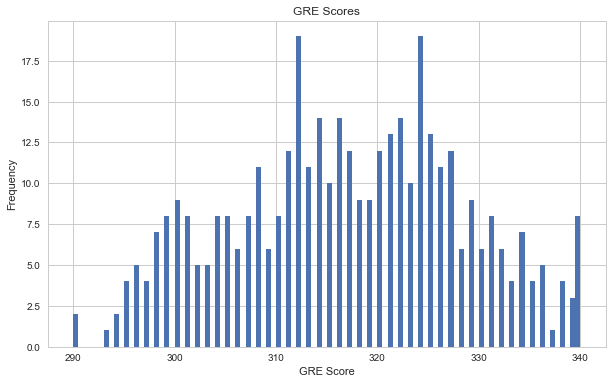
\includegraphics[scale = 0.5]{GRE.png}
    \caption{GRE Distritbution}
\end{figure}
 
 \begin{figure}[H]
 \centering
  \begin{subfigure}[b]{0.45\textwidth}
    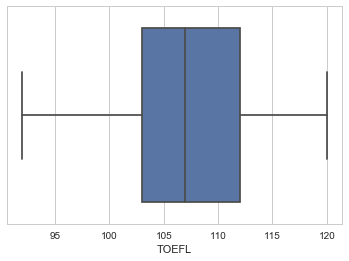
\includegraphics[width=\textwidth]{TOEFL.png}
    \caption{TOEFL Distribution}
    \label{fig:1}
  \end{subfigure}
  %
  \begin{subfigure}[b]{0.45\textwidth}
    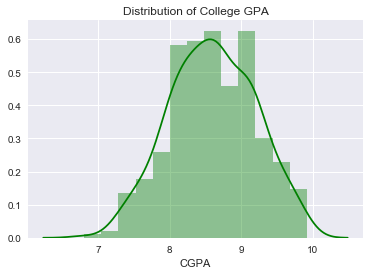
\includegraphics[width=\textwidth]{CGPA.png}
    \caption{CGPA Distribution}
    \label{fig:2}
  \end{subfigure}
\end{figure}
 
\subsection{Regression Methods}

The chance of admission is ranging from 0 to 1 and most variables are continuous, so I decide to build three regression models on the dataset, which are: linear regression model, decision tree regression and random forest regression. Table below presents the $r^2$ value for each model, which is also displayed in Figure 6. Therefore, the linear model predicts most accurately among all three regression models. 

\begin{table}[H]
\centering
\begin{tabular}{|l|l|l|l|}
\hline
Model & Linear Model & Decision Tree & Random Forest \\ \hline
$r^2$ value   & 0.788        & 0.647         & 0.757 \\ \hline
\end{tabular}
\caption{Regression Model Performance}
\end{table}

\begin{figure}[H]
    \centering
    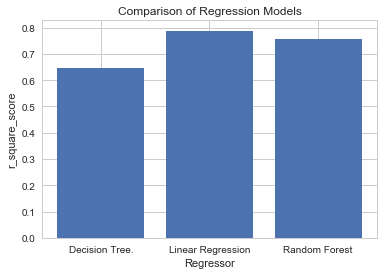
\includegraphics[scale = 0.8]{regression_comparision.png}
    \caption{Regression Models Comparison}
\end{figure}

\subsection{Classification Methods}

Since there are only two results in an application, admitted or rejected, it is also reasonable to user classification methods. According to the distribution of Chance of Admission (Figure 7), I classified COA larger than 0.8 as admitted (COA = 1), and COA = 0 otherwise.
\begin{figure}[H]
    \centering
    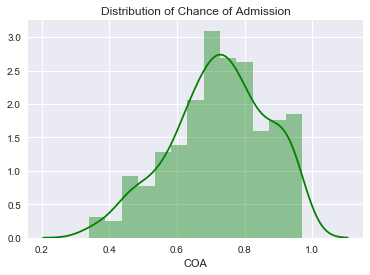
\includegraphics[scale = 0.9]{COA.png}
    \caption{Distribution of Chance of Admission}
\end{figure}

 
 \begin{figure}[H]
 \centering

  \begin{subfigure}[b]{0.48\textwidth}
    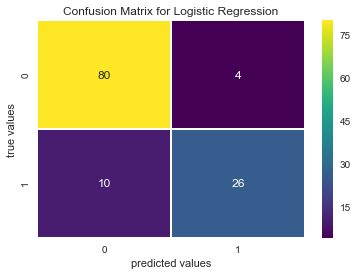
\includegraphics[width=\textwidth]{CM_Logistic_Regression.png}
    \caption{Logistic Regression}
  \end{subfigure}
  %
  \begin{subfigure}[b]{0.48\textwidth}
    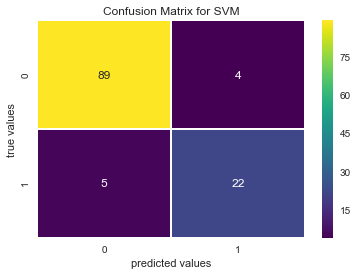
\includegraphics[width=\textwidth]{CM_SVM.png}
    \caption{Support Vector Machine}
  \end{subfigure}
    \begin{subfigure}[b]{0.48\textwidth}
    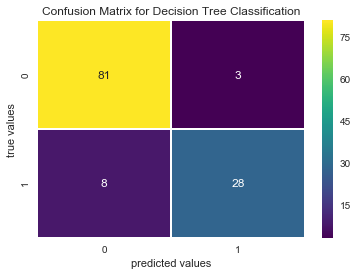
\includegraphics[width=\textwidth]{CM_Decison_Tree.png}
    \caption{Decision Tree}
  \end{subfigure}
  %
  \begin{subfigure}[b]{0.48\textwidth}
    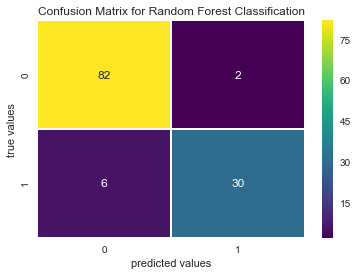
\includegraphics[width=\textwidth]{CM_Random_Forest.png}
    \caption{Random Forest}
  \end{subfigure}
    \begin{subfigure}[b]{0.48\textwidth}
    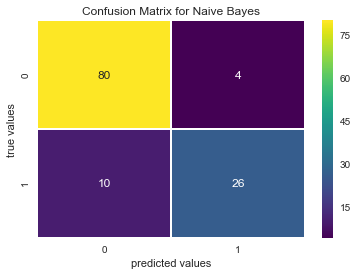
\includegraphics[width=\textwidth]{CM_Naive_Bayes.png}
    \caption{Naive Bayes}
  \end{subfigure}
  %
  \begin{subfigure}[b]{0.48\textwidth}
    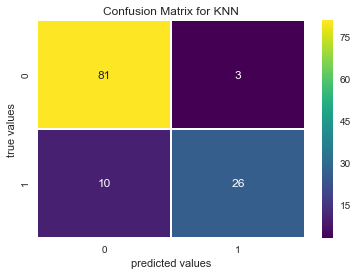
\includegraphics[width=\textwidth]{CM_KNN.png}
    \caption{K Nearest Neighbors}
  \end{subfigure}
   \caption{Confusion Matrices}
\end{figure}

Classification could be evaluated by precision, recall and accuracy score. $Precision = \frac{TP}{TP+FP}$, shows the ability to discriminate false samples.  $Recall = \frac{TP}{TP+FN}$, shows the ability to recognize the true samples. The accuarcy score is also calculated from the confusion matrix, $Accuracy = \frac{TP+TF}{TP+FP+TN+FN}$, could present the overall performance of the models. Table 2 shows the all scores for each classification algorithm I used. And the confusion matrices of each model is presented in Figure 8.

\begin{table}[H]
\centering
\begin{tabular}{|c|c|c|c|c|c|c|}
\hline
Model     & Logistic & SVM   & Naive Bayes & Decision Tree & Random Forest & KNN   \\ \hline
Precision & 0.867    & 0.879 & 0.795       & 0.903         & 0.938         & 0.897 \\ \hline
Recall    & 0.722    & 0.801 & 0.972       & 0.778         & 0.833         & 0.722 \\ \hline
Accuracy  & 0.883    & 0.908 & 0.917       & 0.908         & 0.933         & 0.892 \\ \hline
\end{tabular}
\caption{Classification Methods Performance}
\end{table}
Other than simply use the tools from sklearn packages, there are some little tricks I used. We should always be aware that a decision tree model could be easily over-fitted no matter for regression or classification. Therefore, I set the max depth of tree to be 5 due to multiple experiment results.\\
\begin{lstlisting}[language = Python,frame=shadowbox]
scores = []
for i in range(1,50):
    knn = neighbors.KNeighborsClassifier(n_neighbors=i)
    knn.fit(x_train,y_train_c)
    scores.append(knn.score(x_test,y_test_c))
plt.scatter(range(1,50),scores)
\end{lstlisting}

\begin{figure}[H]
    \centering
    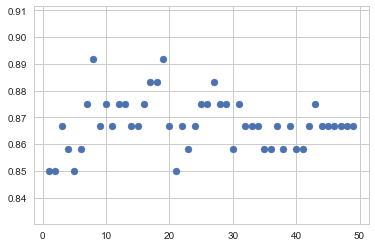
\includegraphics[scale = 0.75]{K_neighbors.png}
    \caption{Scatter Plot to Find K Value}
\end{figure}

For KNN algorithms, users need to set the number of neighbors (k value). I write a simple function to find the best k value to get the highest accuracy score. Figure 9 is the scatter plot generate by the code above. From the scatter plot, K value of 8 leads to the highest accuracy. Therefore, I use k value equals 8 to build the KNN model. \\
The overall compression of these models is visualized in Figure 10. The  criteria used here is the accuracy score. In summary, the Random Forest Classification gets the highest score.
\begin{figure}[H]
    \centering
    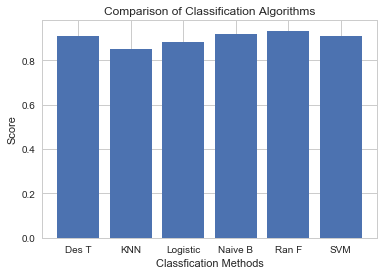
\includegraphics[scale = 1]{classficaiton_comparision.png}
    \caption{Classification Models Comparison}
\end{figure}

\section{Conclusion}

This project analyzes the Graduate Admission dataset in detail. I find that the TOEFL, GRE and College GPA are most important features for admission to the graduate school. The scores of students distributed normally and the students in the upper tail of the normal distribution curve could be more competitive. To predict one's chance of admission there are regression models and classification models available. Linear Regression Model and Random Forest Classification Model are the best models in each categorization. A larger dataset and use of cross-validation could improve the performance of models further. Lastly, I hope this project could help students to find a best fitting graduate school.

\newpage

\section{Reference}

\begin{enumerate}
    \item Mohan S Acharya, Asfia Armaan, Aneeta S Antony : A Comparison of Regression Models for Prediction of Graduate Admissions, IEEE International Conference on Computational Intelligence in Data Science 2019
    \item \url{https://www.tutorialspoint.com/python3/}
    \item \url{https://en.wikipedia.org/wiki/Pandas_(software)}
    \item \url{https://scikit-learn.org/stable/}
    \item \url{https://seaborn.pydata.org/}
\end{enumerate}



\end{sloppypar}
\end{document}